\chapter{Homology}
Before go into what \textit{persistent} homology is, it is well worth our time to clearly state what we mean by homology. Broadly speaking, homology is an invariant of topological spaces which is concerned with cycles in the space which are not boundaries. Or more abstractly, homology captures the notion $n$-dimensional holes in the space. In \textit{persistent} homology we generally work without predefined topological spaces and start with a basic data-set which at most contains some metric structure which we endow with some form of complex. The main complex we will be working with is the simplicial complex, since computationally we can approximate a such a complex on a set of data-points. We will also review homology of cubical complexes as this relates to one of the case studies. Therefore the classical definitions involving concepts such as singular homology are not something we will dwell on, but rather we refer the reader to Hatcher's excellent exposition in \cite{hatcher2002}.


\section{Simplices}
We start with what will constitute our atoms in simplicial homology, namely the simplices.
\begin{definition}[{\cite[p. ~62]{edels}}]
An \textbf{$n$-simplex} is the smallest possible convex set in $\mathbb{R}^{m}$ containing $n+1$ points $v_{0},\dots,v_{n}$ such that the vectors $v_{1}-v_{0}, \dots, v_{n} - v_{0}$ are linearly independent. The points $v_{0},\dots,v_{n}$ are known as the \textbf{vertices} of the simplex. The number $n$ is the \textbf{dimension} of a simplex.
\end{definition}
As seen in Figure \ref{simplices} the $0,1,2$ and $3$-dimensional simplices are familiar shapes consisting of vertices, edges, triangles and tetrahedrons.

\begin{figure}
  \centering
  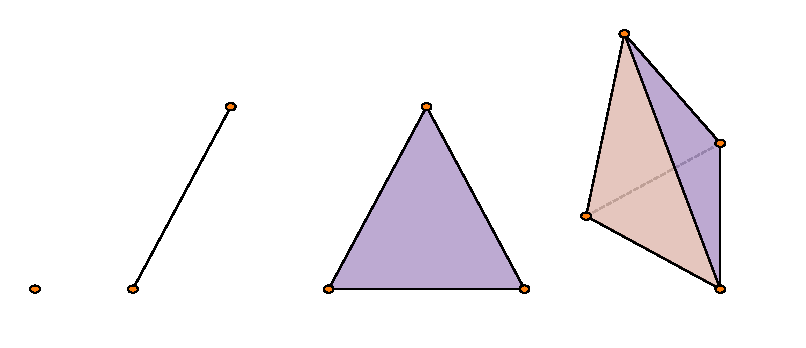
\includegraphics[]{simplex.pdf}
  \caption{
  \label{simplices}
0-simplex (left), 1-simplex (middle left), 2-simplex (middle right) and 3-simplex (right).}
  \end{figure}
\begin{definition}[{\cite[p. ~62]{edels}}]
A \textbf{face} of a simplex is the convex hull of a subset of its vertices. If $\tau$ is a face of $\sigma$ we write $\tau \subseteq \sigma$.
\end{definition}
Since higher dimensional simplices are made up of simplices of lower dimensions we can always decompose a simplex into its faces, in other words the lower dimensional simplices that make up the simplex. For example, a 2-simplex can be decomposed into the three edges that make up the triangle.
\section{Simplicial complex}
By gluing together simplices at their faces as seen in Figure \ref{complex2} we can construct higher-order objects which we call simplicial complexes.
\begin{definition}[{\cite[p. ~63]{edels}}] \label{defsimcomp}
A \textbf{simplicial complex} $K$ is a finite collection of simplices such that

\begin{itemize}
    \item $\sigma \in K$ and $\tau \subset \sigma$ implies that $\tau \in K$
    \item $\sigma_{1}, \sigma_{2} \in K$ implies that $\sigma_{1} \cap \sigma_{2}$ is either empty or a face of both.
\end{itemize}

\end{definition}
The first requirement tells us that a simplicial complex contains the faces of all its simplices. The second requirement tells us that the simplices are only glued together at common faces, in other words we do not allow simplices to intersect other than at their boundary.


We will refer to the construction in Definition \ref{defsimcomp} as a \textbf{geometric simplicial complex}. This is to distinguish it from a simplicial complex where we discard the geometric connotations. It is possible to define a combinatorial simplicial complex by only considering the ordering of the vertices and what higher-dimensional simplices they make up.

\begin{figure}
  \centering
  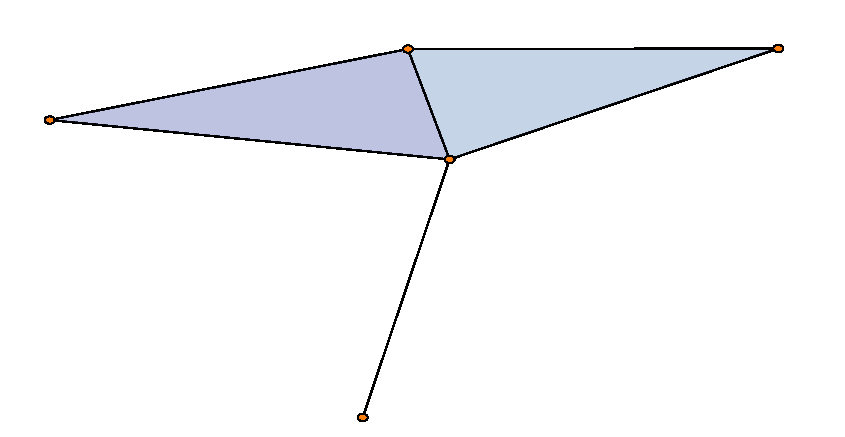
\includegraphics[scale=0.7]{complex.pdf}
  \caption{ \label{complex2} Example of a simplicial complex consisting of two 2-simplices glued together with an attached 1-simplex.}
\end{figure}

\begin{definition}[{\cite[p. ~62]{edels}}]
An \textbf{abstract simplicial complex} $K$ is a finite collection of ordered sets such that $\alpha \in A$ and $\beta \subseteq \alpha$ implies that $\beta \in A$.
\end{definition}

This abstract definition coincides with the geometric definition by calling the elements of $K$ its simplices. The simplices of $K$ are no longer geometric objects in metric space, but simply combinatorial objects consisting of vertex sets.

\begin{definition}
Given a geometric simplicial complex $K$, we can construct an abstract simplicial complex $A$ by translating each simplex $\sigma_{i} \in K$ to the ordered set $[v_{0},\dots,v_{n}]$ where each $v_{i}$ is an algebraic object simply denoting the presence of a vertex. We call $K$ the \textbf{geometric realization} of $A$.
\end{definition}
Hence, we can always transition from a geometric simplicial complex to an abstract simplicial complex. There is an elementary result which allows for the construction in other direction.
\begin{theorem}[{\cite[Geometric Realization Theorem, p. ~64]{edels}}]\label{geometricthm}
Every abstract simplicial complex of dimension $n$ has a geometric realization in $\mathbb{R}^{2d+1}$.
\end{theorem}
Of course, for a given abstract simplicial complex there might be many different ways of giving a geometric realization for it, but at least Theorem \ref{geometricthm} guarantees the existence of one such realization.

From here on we will simply refer to an abstract simplicial complex as a simplicial complex unless stated otherwise. This allows us to state our definitions and work with simplices solely as combinatorial objects.
\section{Simplicial homology}
Roughly speaking, in topology when two spaces homeomorphic they share the same topological properties. One invariant that is the algebraic structure of the higher dimensional holes in the space.
Homology can generally thought of as being the characterization of these holes in a topological space. Beyond that however, it is a way of associating algebraic objects to topological spaces. In the context of simplicial complexes, we first need some algebraic machinery in order to define precisely what we mean by holes in a simplicial complex.

\begin{definition}[\cite{Zomorodian2005}]
  The $k$th \textbf{chain module} $C_{k}(K)$ on a simplicial complex $K$ is the free module with basis given by the $k$-dimensional simplices in $K$ with coefficients in some ring $\mathcal{R}$ with additive unit $0$ and multiplicative unit $1$. In other words, the elements of $C_{k}(K)$ are formal sums
  \[ \sum_{i=1} r_{i}\sigma_{i}\]
  where $r_{i} \in \mathcal{R}$ and $\sigma_{i}$ is a $k$-dimensional simplex in $K$.
\end{definition}
\begin{definition}[{\cite[p. ~2]{weibel1994}}]
  A \textbf{chain complex} $C_{*}$ over a ring $R$ is a family of $R$-modules $\{C_{k}\}_{k
  \in \mathbb{Z}}$ with $R$-module maps $\partial_{k}: C_{k} \to C_{k-1}$ such that the composition $\partial_{k-1} \circ \partial_{k}$ is the zero map. We call the maps $\partial_{k}$ the \textbf{differentials} of the chain complex.
\end{definition}

\begin{theorem}\label{simpchainthm}
Given a simplicial complex $K$ and a ring $\mathcal{R}$ the sequence of chain modules
\begin{center}
\begin{tikzcd}
  \dots \arrow[]{r}{\partial_{k+1}} & C_k(K) \arrow[]{r}{\partial_{k}} & C_{k-1}(K) \arrow[]{r}{\partial_{k-1}} & C_{k-2}(K) \arrow[]{r}{\partial_{k-2}} & \dots \arrow[]{r}{\partial_{1}} & C_0(K)
\end{tikzcd}
\end{center}
with differentials defined as
\begin{align*}
& \partial_{k}:  C_{k}(K) \to C_{k-1}(K) \\
& \partial_{k}(\sigma) =  \sum^{k}_{{i=0}} (-1)^{i} [v_{0},\dots,\hat v_{i}, \dots, v_{k}]
\end{align*}
is a chain complex.
\end{theorem}

\begin{proof}
  All we need to show is that $\partial \partial \sigma = 0 $ for any simplex $\sigma$ and it extends to arbitrary chains since $\partial$ is a homomorphism. By linearity of the homomorphism we get
  \begin{align*}
    \partial \partial \sigma =& \sum_{i} (-1)^{i} \partial [v_{0}, \dots, \hat v_{i}, \dots v_{n}] \\
    =& \sum_{j < i} (-1)^{i} (-1)^{j} [ \dots,  \hat v_{j}, \dots , \hat v_{i}, \dots ] \\ &+ \sum_{i < j} (-1)^{i} (-1)^{j-1}  [ \dots,  \hat v_{i}, \dots , \hat v_{j}, \dots ] \\
    =& 0.
  \end{align*}
  The first sum comes from when $j<i$ since if remove $v_{i}$ the position of $v_{j}$ is unchanged in the resulting simplex, whereas the second sum comes from the other possible case where $i<j$ and so removing $v_{i}$ causes the position of $v_{j}$ to shift by one. Hence, the sums cancel out and so $\partial \partial = 0$. \end{proof}

\begin{example}
Given a simplicial complex $K$ consisting of a triangle without interior as in Figure \ref{trichain}, a chain in $C_{1}(K)$ would be a linear combination of edges. For example, an element of $C_{1}(K)$ is $[v_{0},v_{1}]+[v_{1},v_{2}]$ which is highlighted in green.
\begin{figure}[ht]
  \centering
  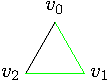
\includegraphics[scale=2]{trichain.pdf}
  \caption{\label{trichain} A simplicial complex in which the 1-chain $[v_{0},v_{1}]+[v_{1},v_{2}]$ is highlighted in green.}
\end{figure}
\end{example}

\begin{example}
Given a $2$-simplex as in Figure \ref{2simplex} we get the differential of the interior of the simplex as \[\partial_{2}([v_{0},v_{1},v_{2}])=[v_{1},v_{2}]-[v_{0},v_{2}]+[v_{1},v_{2}]\] which geometrically is the boundary of the simplex. For this reason we refer to the differential of a chain complex of a simplicial complex as the \textbf{boundary map} or \textbf{boundary operator}.
\begin{figure}[ht]
  \centering
  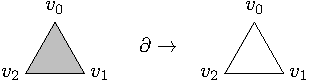
\includegraphics[scale=2]{partialtri.pdf}
  \caption{\label{2simplex} Illustration of how the differential maps a $2$-simplex to its boundary.}
\end{figure}
\end{example}
The notion of the differential being a map from a simplex to its boundary motivates the following definition.
\begin{definition}[{\cite[p. ~4]{weibel1994}}]
  Given a chain complex $C_{*}$ the \textbf{$k$-cycles} $Z_{k}$  and the \textbf{$k$-boundaries} $B_{k}$ of $K$ are the $\mathcal{R}$-modules
  \[ Z_{k} := \ker \partial_{k}\]
  \[ B_{k} := \textrm{im } \partial_{k+1}.\]
  Just as for a chain complex we will sometimes refer to the collection of $Z_{k}$ and $B_{k}$ as $Z_{*}$ or $B_{*}$ respectively.
\end{definition}
Our overarching goal is to characterize $k$-cycles which are not $k$-boundaries. Hence, a vital result is this corollary to Theorem \ref{simpchainthm}.

\begin{corollary}
  The $k$-boundaries are a submodule of the $k$-cycles.
\end{corollary}


\begin{proof}
Let $\sigma \in B_{k} = \textrm{im } \partial_{k+1}$ then for some $\tau \in C_{k+1}$ we have that $\partial_{k+1}(\tau)=\sigma$. Hence,
\[ \partial_{k}(\sigma) = \partial_{k} \partial_{k+1}(\tau) = (\partial_{k} \circ \partial_{k+1}) \tau = 0\]
and so $\sigma \in \ker \partial_{k} = Z_{k}$.
\end{proof}

This tells us that if we can find the cycles and ignore those which are just boundaries, then we have identified the holes. This motivates the following definition of homology.
\begin{definition}
  Given a simplicial chain complex \hspace{0.05cm}$C_{*}$ the homology module $H_{k}$ is defined as
  \[H_{k}(K) := \ker(\partial_{k})/\text{im}(\partial_{k+1})\]
\end{definition}
Hence, the $k$th homology group captures precisely those cycles which are not in the image of the higher dimensional differential. In other words, the non-trivial equivalence classes represent the cycles which are not boundaries.
\begin{example}
Consider the chain complex over $\mathbb{Z}_{2}$ resulting from the simplicial complex in Figure \ref{trihom}.
\begin{figure}[ht]
  \centering
  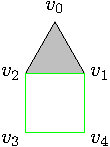
\includegraphics[scale=2]{trisquarefilled.pdf}
  \caption{\label{trihom} }
\end{figure}
There are two 1-cycles, the boundary of the filled triangle and the square. Since the boundary of the filled triangle is in $\text{im} (\partial_{2})$ we get that this element belongs to the trivial class in $H_{1}$. But there is one non-trivial element given by the square without interior. So $H_{1}$ contains one non-trivial element generated by the cycle in green.

To quantify the number of linearly independent generators in a homology module $H_{k}$ we say that the \textbf{$k$th Betti number} is denoted $\beta_{k}$ where $\beta_{k} = \text{rank }(H_{k})$.

\section{Cubical Homology}
The definition we gave of a chain complex is general enough that we need not limit ourselves to chain complexes arising from simplicial complexes. Another type of complex which we can define chain complexes on, and so by extension homology, are cubical complexes. As the atoms of simplicial complexes are simplices, the atoms of cubical complexes are cubes.

\begin{definition}[{\cite[Definition 2.1, p. ~40]{kaczynski2004}}]
An elementary interval is a unit interval $[k,k+1]$ or a degenerate interval $[k,k]$ for $k \in \mathbb{N}$.
\end{definition}

\begin{definition}[{\cite[Definition 2.3-2.4, p. ~40]{kaczynski2004}}]
  An \textbf{elementary cube} $Q$ is the cartesian product of $n$ elementary intervals
  \[Q = \prod^{n}_{i=0} I_{i} \subset \mathbb{R}^{n}\]
  and where $n$ is known as the \textbf{embedding number} $emb(Q)$.
\end{definition}

\begin{definition}[{\cite[Definition 2.4, p. ~41]{kaczynski2004}}]
The \textbf{dimension} $dim(Q)$ of an elementary cube $Q$ is the number of non-degenerate intervals in the product of elementary intervals that make up $Q$.
\end{definition}

Note that under this definition a $0$-dimensional cube is a degenerate elementary interval and a $1$-dimensional cube is a non-degenerate elementary interval. This corresponds to our notion of vertices and edges in simplicial complexes.

We let $\mathcal{K}^{n}$ denote the set of all elementary cubes in $\mathbb{R}^{n}$. The set of all possible elementary cubes is then denote $\mathcal{K}$ defined as
\[ \mathcal{K}:= \bigcup^{\infty}_{n=1} \mathcal{K}^{n} \]
Additionally, we define
\[ \mathcal{K}_{k} := \{ Q \in \mathcal{K} \mid \dim Q = k \}\]
\[ \mathcal{K}^{n}_{k} := \{ \mathcal{K}_{k} \cap \mathcal{K}^{n} \}\]
where it is important to note that $K_{d} \neq K^{d}$ since $K^{d}$ contains any elementary cube embedded in $\mathbb{R}^{d}$. For instance $Q:=[0,0] \times [1,1] \times [2,2] \in \mathcal{K}^{3}$, but $Q \not \in K_{3}$ since $Q$ only consists of degenerate intervals and so $\dim Q = 0$.


\begin{definition}[{\cite[Definition 2.9, p. ~43]{kaczynski2004}}]
  A cubical set $X$ is a finite union of elementary cubes. Given a cubical set $X$ a cubical complex $\mathcal{K}(X)$ is defined as
  \[ \mathcal{K}(X):= \{Q \in \mathcal{K} \mid Q \subset X\}.\]
  Additionally we define the $k$-skeleton of the cubical complex as
  \[ \mathcal{K}_{k}(X):= \{ Q \in \mathcal{K}(X) \mid \dim Q = k \}.\]
\end{definition}

Much like in the case with the simplicial complexes, working with the actual geometric objects can be unwieldy when doing algebraic calculations. For this reason we introduce an abstract object for each elementary cube, called an elementary chain.
\begin{definition}[{\cite[p. ~48]{kaczynski2004}}]
  Given a cube $Q \in \mathcal{K}^{n}_{k}$ the elementary $k$-chain $\hat Q$ is a map
  \[\hat Q: \mathcal{K}^{n}_{k} \to \mathbb{Z}\]
\end{definition}

Furthermore, since elementary cubes consist of finite cartesian products of elementary intervals, we need a corresponding notion on elementary chains.

\begin{definition}[{\cite[Definition 2.23, p. ~51]{kaczynski2004}}]
Given two elementary cubes $P,Q$ The cubical product is defined as \[\hat P \diamond \hat Q:= \widehat{P \times Q}\]
\end{definition}
Fix some ring $\mathcal{R}$ with additive unit $0$ and multiplicative unit $1$ and then we can proceed as for the simplicial case.
\begin{definition}[{\cite[Definition 2.27, p. ~53]{kaczynski2004}}]
  The \textbf{$k$th chain module} of a cubical complex $\mathcal{K}(X)$ is the free $R$-module $C_{k}(\mathcal{K}(X))$ whose elements are formal sums
  \[ \sum \alpha_{i} Q_{i}\]
  known as \textbf{$k$-chains} where $\alpha_{i} \in \mathcal{R}$ and $Q_{i} \in K_{k}(X)$.
\end{definition}

The cubical product extends to $k$-chains in the following way.

\begin{definition}
The cubical product $\diamond$ of two $k$-chains $c_{1},c_{2}$ of a chain module on a cubical complex is \[ c_{1} \diamond c_{2} = \sum_{i} \sum_{j} \alpha_{i} \beta_{j} \hat P_{i} \diamond  \hat Q_{j}\]
\end{definition}

It can be shown with relative ease that the cubical product on $k$-chains is distributive, associative and is equal to 0 if one of its arguments is 0, see \cite[Proposition 2.25, p. ~51]{kaczynski2004}.

All we need to do in order for the machinery of homology to be applicable is to define a boundary operator on the elements of the chain modules of a cubical complex which has the property that $\partial \partial = 0$.
\begin{definition}[{\cite[Definition 2.31, p. ~54]{kaczynski2004}}]
  The boundary map of an elementary cube is defined inductively on the embedding number cube in the following way. Let $Q$ be an elementary cube, we then have that
  \[ \partial \hat Q =
    \begin{cases}
      0 & Q = [k,k] \\
      \widehat{[k+1,k+1]} - \widehat{[k,k]} & Q = [k,k+1] \\
      \partial \hat I \diamond \hat P +(-1)^{\dim \hat I} \hat I \diamond \partial \hat P & Q=I \times P, emb(Q) \geq 2
    \end{cases}
  \]
  which extends linearly on $k$-chains.
\end{definition}
\begin{theorem}[{\cite[Proposition 2.37, p. ~58]{kaczynski2004}}]
The composed boundary map $\partial \partial$ is the zero map.
\end{theorem}
\begin{proof}
  Let $Q$ be an elementary cube. If $emb(Q)=0$ then by the definition of the boundary map $\partial (\partial Q) = \partial(0) = 0$. If $emb(Q)=1$ then
  \begin{align*}
    \partial \partial Q =& \partial([k+1,k+1]-[k,k]) \\ =&\partial([k+1,k+1])-\partial([k,k])
                                                          \\=&0-0\\=&0
  \end{align*}
We prove it for higher embedding numbers by induction. Assume it holds for $emb(Q)=n$, we want to prove that it also holds for $emb(Q)=n+1$.
\begin{align*}
  \partial \partial Q =& \partial(\partial \hat I \diamond \hat P) + \partial((-1)^{\dim I} \hat I \diamond \partial \hat P)
\end{align*}
Now assume that $\dim I = 0$ then $I$ is a degenerate interval and so we get
\begin{align*}
  \partial \partial Q =& \partial(0 \diamond \hat P) + \partial((-1)^{0} \hat I \diamond \partial \hat P) \\
  =& 0 + \partial( \hat I \diamond \partial \hat P) \\
  =& (\partial \hat I \diamond \partial \hat P + (-1)^{\dim I} \hat I \circ \partial \partial \hat P \\
  =& 0 + \hat I \diamond \partial \partial \hat P \\
  =& 0 + 0 \\
  =& 0
\end{align*}
where $\partial \partial \hat P = 0$ follows from the induction hypothesis since $\dim \hat P = n+1-1=n$. Now, let us assume the other case, namely that $\dim I = 1$ then we get
\begin{align*}
\partial \partial Q =& \partial(\partial \hat I \diamond \hat P) - \partial( \hat I \diamond \partial \hat P)\\
=& \partial \partial \hat I \diamond \hat P + (-1)^{\dim \partial I} \partial \hat I \diamond \partial \hat P - (\hat \partial I \diamond \partial \hat P - \hat I \diamond \partial \partial \hat P)\\
=& 0 + (-1)^{\dim \partial \hat I} \partial \hat I \diamond \partial \hat P - (\hat \partial I \diamond \partial \hat P - 0)\\
  =& \partial \hat I \diamond \partial \hat P - \partial \hat I \diamond \partial \hat P\\
  =& 0
\end{align*}
where $\dim \partial \hat I = 0$ since $ I$ is an elementary interval. Since we have now shown the induction hypothesis holds for $n+1$ given it holds for $n$, this concludes the proof by induction.
\end{proof}
We now have everything we need to construct a chain complex on cubical complexes: a sequence of $\mathcal{R}$-modules, the $k$-chain modules on cubical complexes, and module homomorphisms $\partial$ which have the property of $\partial \partial = 0$. Since our prior definitions with regards to \textit{homology} were entirely stated in terms of chain complexes we can be assured that homology on chain complexes given by cubical complexes is well-defined.

%%% Local Variables:
%%% mode: latex
%%% TeX-master: "thesis.tex"
%%% End:
